
%\newpage
\appendix

%	In the following appendices we will prove the bounds based on the events $\xi_{1}$,$\xi_{2}$ and $\xi_{3}$. In $\xi_{1}$, we will assume two important assumptions $i)\hat{r}^{*}<\hat{r}_{i},\forall i\in s_{i}$ and $ii)\exists a_{i}\in s_{i}$ such that $\sqrt{\dfrac{\epsilon_{m}}{w_{s_{i}}}}<\dfrac{\Delta_{i}}{5}$. For $\xi_{2}$, we will assume that $a^{*}\in s^{*}$ and $|s^{*}|=1$, $a_{i}\in s_{i} \forall a_{i}\setminus a^{*}\in B_{m}$ and $\exists a_{max_{s_{i}}}$ such that $\sqrt{\epsilon_{m}}<\dfrac{2\Delta_{s}}{5}$, where $\Delta_{s}=r^{*}-r_{max_{s_{i}}}$ and $\hat{r}_{max_{s_{i}}}>\hat{r}_{i}, \forall i\in s_{i}$. $\xi_{3}$ be the event when the optimal arm $a^{*}$ gets eliminated by a sub-optimal arm. At the start of any round $m$, we fix $\epsilon_{m}$.

%\todos{(Subho) Took $\psi(m)=1$, removed $w_{s_{i}}$ from proofs. Here, $\epsilon_{m}$ is now the $\tilde{\Delta}_{m}$ of Ucb-Revisited}


%\section{Appendix A}
%\begin{proposition}
%The probability that the optimal arm $a^{*}\in s_{i}$ will lie above $\hat{r}_{min_{s_{i}}}+ \dfrac{\hat{\Delta}_{s_{i}}}{2}$ after $\bigg\lceil\dfrac{2\log (T\epsilon_{m}^{2})}{\epsilon_{m}}\bigg\rceil$ pulls in the $m$-th round is given by $\bigg\lbrace 1- \dfrac{1}{(T\epsilon_{m}^{2})^{\ell_{m}^{2}\epsilon_{m}}} \bigg\rbrace$ where $\hat{r}_{min_{s_{i}}}$ is the minimum payoff in $s_{i}$, $\hat{\Delta}_{s_{i}}=max_{i\in s_{i}}\hat{r}_{i}-min_{j\in s_{i}}\hat{r}_{j}, i\neq j$, $\epsilon_{m}$ is halved after every round and $T$ is the horizon. 
%\end{proposition}
%
%%$\epsilon_{m}=\max{\bigg\lbrace\dfrac{\hat{\Delta}_{m}}{\ell_{m}} \dfrac{2}{\sqrt{\psi{(m)T}}}\bigg\rbrace}$
%
%\begin{proof} of Proposition 1:
%\newline
%We start by considering the worst case scenario that in the $m$-th round, in a cluster $s_{i}$, the optimal arm $a^{*}$ has performed worst, such that $\hat{r}^{*}<\hat{r}_{i},\forall a_{i} \in s_{i}$. Let, $\hat{\Delta}_{s_{i}}=max_{i\in s_{i}}\hat{r}_{i}-min_{j\in s_{i}}\hat{r}_{j}$ where $i\neq j$. Also, let $|s_{i}|=k_{s_{i}}$ and $\hat{r}^{*}=\hat{r}_{min_{s_{i}}}\leq\hat{r}_{i},\forall i\in s_{i}$ also $\hat{r}_{max_{s_{i}}}\geq\hat{r}_{i},\forall i\in s_{i}$.
%\newline
%%Now, we have to bound the $\mathbb{P}\lbrace\hat{r}^{*}\geq\hat{r}_{max_{s_{i}}} - \hat{\Delta}_{s_{i}}\rbrace$
%%%\leq U_{m}$, where $U_{m}$ is an upper bound.
%%\newline
%Again, given that there are $k_{s_{i}}$ number of arms in $s_{i}$, and for each $a_{i},a_{j}\in s_{i}$ since $|\hat{r}_{i}-\hat{r}_{j}|\leq\epsilon_{m}$, the longest possible gap is $(k_{s_{i}}-1)\epsilon_{m}$ which is greater than the actual estimated gap $\hat{\Delta}_{s_{i}}$.
%\newline
%So, $\hat{\Delta}_{s_{i}}\leq (k_{s_{i}}-1)\epsilon_{m}$, as $|\hat{r}_{i}-\hat{r}_{j}|\leq\epsilon_{m}, \forall i,j \in s_{i}$
%\newline\hspace*{3.5em}$\leq \ell_{m}\epsilon_{m}$, as $k_{s_{i}}\leq \ell_{m}$
%%\newline Again in $\xi_{1}$, $\hat{\Delta}_{s_{i}}\geq \epsilon_{m}$, for sufficiently large $\ell_{m}$, as $\epsilon_{m}=\dfrac{\hat{\Delta}_{s,m}}{\ell_{m}}$, where $\hat{\Delta}_{s,m}=\max_{i\in B_{m}}{\hat{r}_{i}}-\min_{j\in B_{m}}{\hat{r}_{j}},i\neq j$ and $\ell_{m}$ is doubled after every round.
%%$\mathbb{P}\lbrace\hat{r}^{*}\geq\hat{r}_{m}+ \dfrac{\hat{\Delta}_{s_{i}}}{2}\rbrace=
%%\newline\hspace*{0em} $\mathbb{P}\lbrace\hat{r}^{*}\geq\hat{r}_{max_{s_{i}}} - \hat{\Delta}_{s_{i}}\rbrace\Rightarrow\mathbb{P}\lbrace\hat{r}^{*}+\dfrac{\hat{\Delta}_{s_{i}}}{2}\geq\hat{r}_{max_{s_{i}}} - \dfrac{\hat{\Delta}_{s_{i}}}{2}\rbrace$
%%\leq U_{m}$ .
%%\newline But we know that $r^{*}>r_{s}$ and we know that in $\xi_{1}$, $a_{s}$ has performed such that $\hat{r}_{s} \leq r^{*}$.
%\newline Now, applying Chernoff-Hoeffding bound and considering independence of events,
%\newline $\mathbb{P}\lbrace\hat{r}^{*}\leq{r}^{*} + \dfrac{\hat{\Delta}_{s_{i}}}{2}\rbrace\Rightarrow \mathbb{P}\lbrace\hat{r}^{*}\leq{r}^{*} + \dfrac{\ell_{m}\epsilon_{m}}{2}\rbrace $
%%exp(-2 \dfrac{\hat{\Delta}_{s_{i}}^{2}}{4}n^{*})$
%%\newline\hspace*{8em}
%$\leq exp(-2\dfrac{(\ell_{m}\epsilon_{m})^{2}}{4} n^{*})$
%%as $\hat{\Delta}_{s_{i}}\geq \epsilon$
%%\newline For simplicity we will take $\psi(m)=1$
%\newline Now, putting $n_{m}=n^{*}=\dfrac{2\log (T\epsilon_{m}^{2})}{\epsilon_{m}}$
%\newline$\mathbb{P}\lbrace\hat{r}^{*}\leq{r}^{*} +  \dfrac{\ell_{m}\epsilon_{m}}{2}\rbrace\leq exp(-\ell_{m}^{2}\epsilon_{m} \log(T\epsilon_{m}^{2}))$
%%\leq exp(-\hat{\Delta}_{s_{i}} \log(\psi(m)T\epsilon_{m}^{2}))
%%\newline Now, $w_{s_{i}}=k_{s_{i}}D\leq$
%%\newline\hspace*{8em}$\leq exp(-\ell_{m}^{2}\epsilon \log(4\psi(m)T\epsilon_{m}^{2}))$
%%as $\dfrac{1}{w\ell_{m}}< \hat{\Delta}_{s_{i}}, \forall m\in {1,2,..,\lceil\log T\rceil}$
%\newline $\mathbb{P}\lbrace\hat{r}^{*}\leq{r}^{*} +  \dfrac{\ell_{m}\epsilon_{m}}{2}\rbrace\leq \dfrac{1}{(T\epsilon_{m}^{2})^{\ell_{m}^{2}\epsilon_{m}}}$
%%\leq \dfrac{1}{(4\psi(m)T\epsilon_{m}^{2})^{\ell_{m}^{2}\Delta}}$, as $\forall m, \epsilon_{m}\geq \Delta$
%\newline
%%Similarly, $\mathbb{P}\lbrace\hat{r}_{max_{s_{i}}}\geq{r}_{max_{s_{i}}} -  \dfrac{\ell_{m}\epsilon_{m}}{2}\rbrace\leq \dfrac{1}{(\psi(m)T\epsilon_{m}^{2})^{\ell_{m}^{2}\epsilon_{m}}}$
%%as $\forall m, \epsilon_{m}\geq \Delta$
%%\newline
%Hence, the probability that the optimal arm $a^{*}$ after $n_{m}$ pulls going above $\hat{r}_{min_{s_{i}}}+\dfrac{\hat{\Delta}_{s_{i}}}{2}$ is $\bigg\lbrace 1- \dfrac{1}{(T\epsilon_{m}^{2})^{\ell_{m}^{2}\epsilon_{m}}} \bigg\rbrace$
%
%\end{proof}

%\begin{figure}[!tbp]
%\centering
%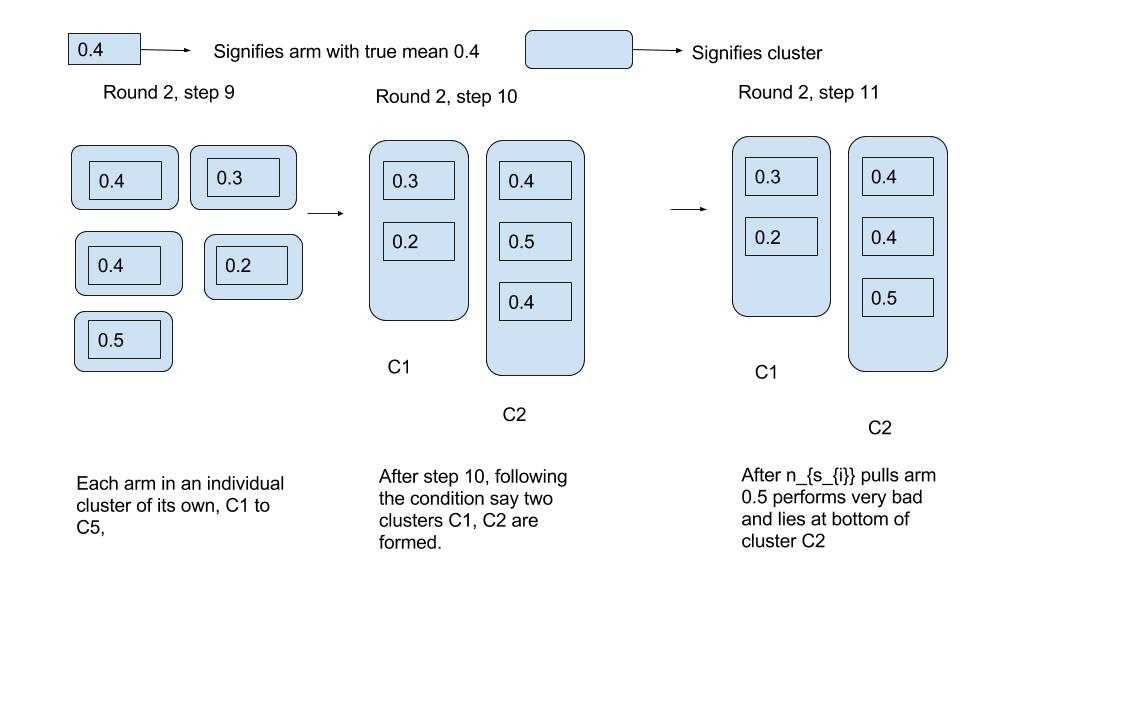
\includegraphics[scale=0.4]{img/diag1.jpg}
%\caption{Steps 9-11}
%\end{figure}
%\begin{figure}[!tbp]
%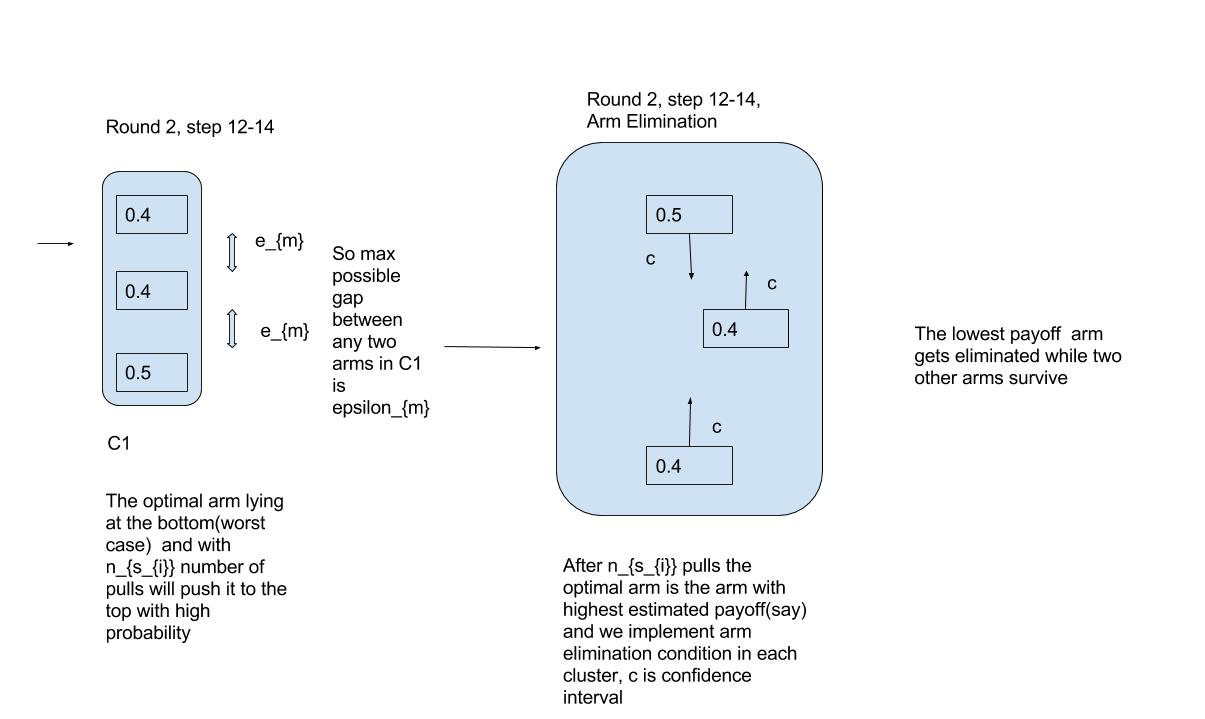
\includegraphics[scale=0.4]{img/diag2.jpg}
%\caption{Steps 12-14}
%\end{figure}
%\begin{figure}[!tbp]
%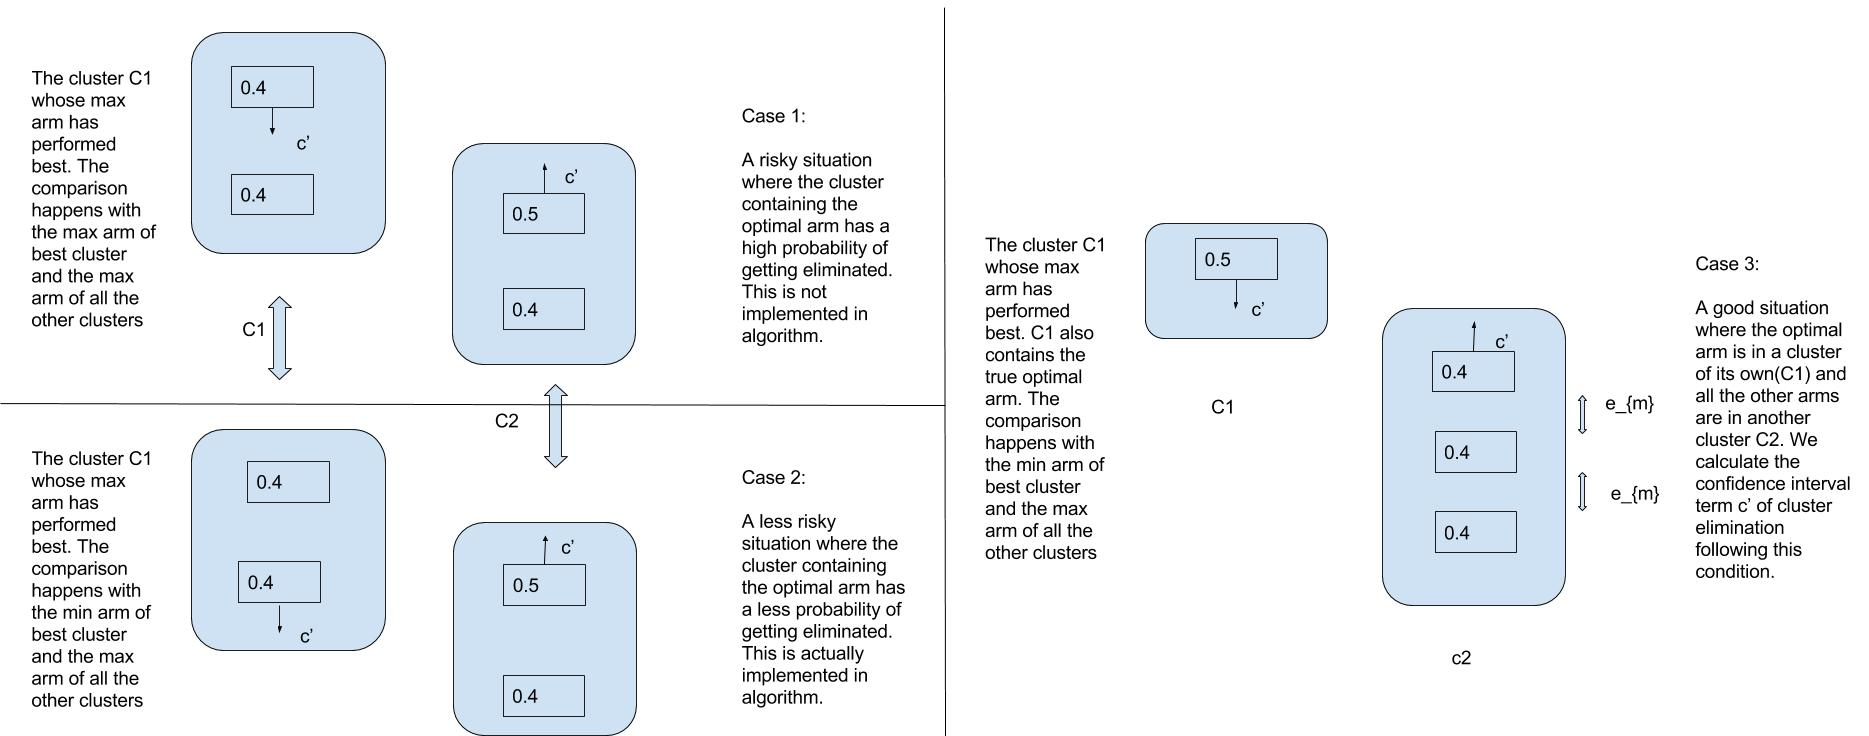
\includegraphics[scale=0.25]{img/diag3.jpg}
%\caption{Different scenarios of Cluster Elimination}
%\end{figure}




\section{Appendix A}
\begin{proposition}
Considering only the arm elimination condition, the total regret till $T$ is upper bounded by $R_{T}\leq \sum_{i\in A:\Delta_{i}\geq b}\bigg \lbrace \bigg(\dfrac{44}{(\Delta_{i})^{3}}\bigg) + \bigg(\Delta_{i}+\dfrac{32\log{(T\dfrac{\Delta_{i}^{4}}{16})}}{\Delta_{i}}\bigg)\bigg\rbrace + \sum_{i\in A:0\leq\Delta_{i}\leq b}\dfrac{12}{b^{3}} + max_{i:\Delta\leq b}\Delta_{i}T$, where $T$ is the horizon.
\end{proposition}

\begin{proof} of Proposition 5:

Let, $\rho_{a}=1$ and for each sub-optimal arm $a_{i}$, $m_{i}=\min{\lbrace m|\sqrt{\epsilon_{m}}\leq \dfrac{\Delta_{i}}{2} \rbrace}$ be the first round when $\sqrt{\epsilon_{m}}\leq \dfrac{\Delta_{i}}{2}$.

\subsection{Case a:} 
Some sub-optimal arm $a_{i}$ is not eliminated in round $m_{i}$ or before and the optimal arm $a^{*}\in B_{m_{i}}$
\newline In arm elimination condition, given the choice of confidence interval $c_{m}$, we want to bound the event $\hat{r}_{i}+c_{m_{i}}\leq \hat{r}^{*}-c_{m_{i}}$. 
%In this proof we will consider $w_{s_{i}}=1$ and $\psi(m)=1$. 
%Later, we will discuss how different values of $w_{s_{i}}$ actually effects the regret bound.
%with a more tighter event of $ \hat{r}_{i} + \sqrt{w_{s_{i}}}c_{m} \leq \hat{r}^{*} - \sqrt{w_{s_{i}}}c_{m}$ which will result in faster elimination of arms within a cluster, given the choice of $c_{m}$ and $w_{s_{i}}$.
\newline Now, $c_{m_{i}}=\sqrt{\dfrac{\log (T\epsilon_{m_{i}}^{2})}{2 n_{m_{i}}}}$.
\newline Putting the value of $n_{m_{i}}=\dfrac{2\log{(T\epsilon_{m_{i}}^{2})}}{\epsilon_{m_{i}}}$ in $c_{m_{i}}$,
\newline $c_{m_{i}}=\sqrt{\dfrac{\epsilon_{m_{i}}\log (T\epsilon_{m_{i}}^{2})}{2*2 \log(T\epsilon_{m_{i}}^{2})}}=\dfrac{\sqrt{\epsilon_{m_{i}}}}{2} = \sqrt{\epsilon_{m_{i}+1}} < \dfrac{\Delta_{i}}{4} $
%\leq\dfrac{\epsilon_{m}\sqrt{\ell_{m}}}{2\sqrt{w\ell_{m}}}\leq \dfrac{\epsilon_{m}}{2\sqrt{w}}$.
%\newline But in $\xi_{1}$, $\ell_{m}=2^{m}$.
%\newline Hence, $c\leq \dfrac{\epsilon_{m} 2^{m/2}}{4}$.
\newline Again, $\exists a_{i} \in s_{i}$ such that, 
$\hat{r}_{i} + c_{m_{i}}\leq r_{i} + 2c_{m_{i}} $
%\newline\hspace*{14em}$= \hat{r}_{i}-\sqrt{\epsilon_{m}} + 2c_{m} +\sqrt{\epsilon_{m}}$
\newline\hspace*{14em}$= \hat{r}_{i} + 4c_{m_{i}} - 2c_{m_{i}} $
\newline\hspace*{14em}$\leq r_{i} + \Delta_{i} - 2c_{m_{i}}$
\newline\hspace*{14em}$< r^{*} -2c_{m_{i}} $
\newline\hspace*{14em}$\leq \hat{r}^{*} - c_{m_{i}}$
%\newline\hspace*{14em}$= r_{i} + 5\dfrac{\sqrt{\epsilon_{m}}}{\sqrt{w_{s_{i}}}} - 2\sqrt{w_{s_{i}}}c_{m}$
%\newline \hspace*{4em}
%\newline But, $\epsilon_{m}=\dfrac{\hat{\Delta}_{s,m}}{\ell_{m}}$, where $\hat{\Delta}_{s,m}=\max_{i\in B_{m}}{\hat{r}_{i}}-\min_{j\in B_{m}}{\hat{r}_{j}},i\neq j$ and $\ell_{m}$ is increased after every round.
%\newline \hspace*{4em}$\leq \hat{r}_{i} + \epsilon_{m} 2^{(m-4)/2} - 2c$
\newline Hence, we get that as soon as $\sqrt{\epsilon_{m_{i}}}<\dfrac{\Delta_{i}}{2}$, $\exists a_{i}$ which gets eliminated.
%\newline So, $\hat{r}_{i}+c_{m}\leq \hat{r}_{i}+2c_{m}\leq r_{i} + \Delta_{i} - 2\sqrt{w_{s_{i}}}c_{m}\leq r^{*} - 2\sqrt{w_{s_{i}}}c_{m}$
%\leq \hat{r}^{*} - \sqrt{w}c_{m}
%\newline $\Rightarrow\hat{r}_{i}+c_{m}\leq \hat{r}_{i} - \sqrt{w}c_{m}  \leq r^{*} - \sqrt{w}c_{m}$
%\newline $\Rightarrow \hat{r}_{i} \leq {r}^{*} - 2\sqrt{w_{s_{i}}}c_{m} - 2c_{m} \leq \hat{r}^{*} - 2\sqrt{w_{s_{i}}}c_{m}$
\newline So, we need to bound the event of $\hat{r}_{i}+c_{m_{i}}\leq \hat{r}^{*}-c_{m_{i}}$ given that $\sqrt{\epsilon_{m_{i}}}<\dfrac{\Delta_{i}}{2}$ becomes true for some arm $a_{i}$ after the $m$-th round and $c_{m}=\sqrt{\dfrac{\log (T\epsilon_{m_{i}}^{2})}{2 n_{m_{i}}}}$.
%\newline $\Rightarrow \hat{r}_{i}+2c_{m}\leq \hat{r}_{i} + 2\sqrt{w}c_{m} \leq \hat{r}^{*}$
%\newline $\Rightarrow \hat{r}_{i} + \sqrt{w}c_{m} \leq \hat{r}^{*} - \sqrt{w}c_{m}$
%\newline $\Rightarrow\hat{r}_{i}+c_{m}\sqrt{\dfrac{w\ell_{m}}{\epsilon_{m}}} \leq \hat{r}^{*}-c_{m}\sqrt{\dfrac{w\ell_{m}}{\epsilon_{m}}} $, as $c_{m}\sqrt{\dfrac{w\ell_{m}}{\epsilon_{m}}} > 0$

%\begin{proof} of Proposition 2:
%\newline
%Now, we can bound $\hat{r}_{i}+c_{m}\leq \hat{r}^{*}-c_{m}$ given that $\sqrt{\epsilon_{m}}<\dfrac{\Delta_{i}}{2}$ for some arm $a_{i}\in s_{i}$. 
	So, we need to bound the probability,
\newline\hspace*{4em} $\mathbb{P}\lbrace\hat{r}^{*}\leq r^{*} - c_{m_{i}}\rbrace\leq U_{m}$, where $U_{m}$ is an  arbitrary upper bound.
%, for a fixed $n_{s_{i}}$.
%\mathbb{P}\lbrace\hat{r}^{*}\leq r^{*} - c_{m}\rbrace\leq
\newline
%Here, we guarantee that only if $\hat{r}^{*}\leq r^{*} - c_{m}\sqrt{\dfrac{w\ell_{m}}{\epsilon_{m}}}$ or $\hat{r}_{i}\geq r_{i} + c_{m}\sqrt{\dfrac{w\ell_{m}}{\epsilon_{m}}}$ then only arm will not be deleted. This is a more aggressive arm elimination condition than simply looking at $\hat{r}^{*}\leq r^{*} - c_{m}$ or $\hat{r}_{i}\geq r_{i} + c_{m}$ because we are exploring much carefully by dividing the larger problem into sub-problems.
%\newline
Applying Chernoff-Hoeffding bound and considering independence of events,
\newline
\newline\hspace*{0em} $\mathbb{P}\lbrace\hat{r}^{*}\leq r^{*} - c_{m_{i}}\rbrace\leq exp(-2c_{m_{i}}^{2}n_{m_{i}})$
\newline\hspace*{8em} $\leq exp(-2 * \dfrac{\log (T\epsilon_{m_{i}}^{2})}{2 n_{m_{i}}} *n_{m_{i}})$
\newline\hspace*{8em} $\leq \dfrac{1}{T\epsilon_{m_{i}}^{2}}$
%$\leq \bigg(\dfrac{1}{4\psi(m)T\epsilon_{m}^{2}}\bigg)^{D}$, as $\ell_{m}-1\leq D$
%\newline\hspace*{2em}
\newline
Similarly, $\mathbb{P}\lbrace\hat{r}_{i}\geq r_{i} + c_{m_{i}}\rbrace\leq \dfrac{1}{T\epsilon_{m_{i}}^{2}}$
\newline
Summing, the two up, the probability that a sub-optimal arm $a_{i}$ is not eliminated in $m_{i}$-th round is  $\bigg(\dfrac{2}{T\epsilon_{m_{i}}^{2}}\bigg)$. 
\newline
Summing up over all arms in $A$ and bounding trivially by $T\Delta_{i}$,
%\sum_{i\in A}\bigg(\dfrac{2}{T\epsilon_{m_{i}}^{2}}\bigg)\leq
\newline\hspace*{4em} $\sum_{i\in A}\bigg(\dfrac{2T\Delta_{i}}{T\epsilon_{m_{i}}\dfrac{\Delta_{i}}{2}^{4}}\bigg)\leq \sum_{i\in A}\bigg(\dfrac{8}{\epsilon_{m_{i}}\Delta_{i}}\bigg)\leq \sum_{i\in A}\bigg(\dfrac{32}{\Delta_{i}^{3}}\bigg)$


\subsection{Case b1:} 
Either an arm $a_{i}$ is eliminated in round $m_{i}$ or before or else there is no optimal arm $a^{*}\in B_{m_{i}}$.
\newline
Also, since we are eliminating a sub-optimal arm $a_{i}$ on or before round $m_{i}$, it is pulled no longer than,
\newline
\hspace*{4em}$n_{m_{i}}=\bigg\lceil\dfrac{2\log{(T\epsilon_{m_{i}}^{2})}}{\epsilon_{m_{i}}}\bigg\rceil$
\newline
%$\sqrt{\dfrac{\epsilon_{m}}{w}}<\dfrac{\Delta_{i}}{5}\Rightarrow \sqrt{\dfrac{\epsilon_{m}}{\ell_{m}^{2}}}<\dfrac{\Delta_{i}}{5}$, as $w\geq \ell_{m}^{2}$
%\newline
%$\Rightarrow \sqrt{\dfrac{\epsilon_{m}}{\ell_{m}^{2}}}<\dfrac{\Delta_{i}}{5}$
%\newline
So, the total contribution of $a_{i}$  till round $m_{i}$ is given by,
\newline
\hspace*{4em}$\Delta_{i}\bigg\lceil\dfrac{2\log{(T\epsilon_{m_{i}}^{2})}}{\epsilon_{m_{i}}}\bigg\rceil$
%\newline
%\hspace*{4em}
$\leq\Delta_{i}\bigg\lceil\dfrac{2\log{(T(\dfrac{\Delta_{i}}{2})^{4})}}{(\dfrac{\Delta_{i}}{2})^{2}}\bigg\rceil$, since $\sqrt{\epsilon_{m_{i}}}\leq\dfrac{\Delta_{i}}{2}$
\newline
\hspace*{12em}
$\leq\Delta_{i}\bigg(1+\dfrac{32\log{(T(\dfrac{\Delta_{i}}{2})^{4})}}{\Delta_{i}^{2}}\bigg)$
\newline
\hspace*{12em}
$\leq\Delta_{i}\bigg(1+\dfrac{32\log{(T\dfrac{\Delta_{i}^{4}}{16})}}{\Delta_{i}^{2}}\bigg)$
\newline
Summing over all arms,
\newline
\hspace*{4em}$\leq\sum_{i\in A}\Delta_{i}\bigg(1+\dfrac{32\log{(T\dfrac{\Delta_{i}^{4}}{16}})}{\Delta_{i}^{2}}\bigg)$
%\newline
%\hspace*{4em}$\leq\sum_{i\in B_{m}}\bigg(\Delta_{i}+\dfrac{27\log{(\psi(m)T\dfrac{\Delta_{i}^{\frac{8}{5}}}{12})}}{\Delta_{i}^{\frac{3}{5}}}\bigg)$
%\newline
%\hspace*{4em}$\leq\sum_{i\in B_{m}}\bigg(\Delta_{i}+\dfrac{12.5\log{(\psi(m)T\Delta_{i}^{4})}}{\Delta_{i}}\bigg)$
	%Thus, we see that the growth of the $n_{s_{i}}$ is always linear and not quadratic as in UCB-Revisited(\cite{auer2010ucb}). Also once $2l_{m}=D$, then $n_{s_{i}}$ will remain constant for the next rounds till stopping condition is met. Thus we have a more controlled exploration than UCB-Revisited(\cite{auer2010ucb}) and Median Elimination(\cite{even2006action}). Hence, 
%\newline
%\hspace*{4em}$\leq\sum_{i\in B_{m}}\bigg(\Delta_{i}+\dfrac{54\log{(\psi(m)T\dfrac{\Delta_{i}^{\frac{8}{5}}}{12})}}{\Delta_{i}^{\frac{3}{5}}}\bigg)$
%\newline
%But, $\psi(m)\leq c/m$ for any $c>0$ and so the regret upper bound comes off as 
%But, $\psi(m) = 1$ the regret upper bound comes off as 
%\newline
%$R_{T}\leq \sum_{i\in A}\bigg (\max{\bigg\lbrace \bigg(\dfrac{32}{(\Delta_{i})^{3}}\bigg) ,\bigg(\dfrac{25\Delta_{i}}{(\Delta^{2})(0.16T\Delta^{2})^{2|B_{m}|^{2}\Delta/5}}\bigg)\bigg\rbrace} + \bigg(\Delta_{i}+\dfrac{32\log{(T\dfrac{\Delta_{i}^{4}}{16})}}{\Delta_{i}}\bigg)\bigg)$. 

\subsection{case b2:} 
In this case we will consider that the optimal arm $a^{*}$ was eliminated by a sub-optimal arm. Firstly, if conditions of case b1 holds then the optimal arm $a^{*}$ will not be eliminated in round $m=m_{*}$ or it will lead to the contradiction that $r_{i}>r^{*}$. In any round $m_{*}$, if the optimal arm $a^{*}$ gets eliminated then for any round from $1$ to $m_{j}$ all arms $a_{j}$ such that $\sqrt{\epsilon_{m}}<\dfrac{\Delta_{j}}{2}$ were eliminated according to assumption in case b1. Let, the arms surviving till $m_{*}$ round be denoted by $A^{'}$. This leaves any arm $a_{b}$ such that $\sqrt{\epsilon_{m}}\geq\dfrac{\Delta_{b}}{2}$ to still survive and eliminate arm $a^{*}$ in round $m_{*}$. Let, such arms that survive $a^{*}$ belong to $A^{''}$. Also maximal regret per step after eliminating $a^{*}$ is the maximal $\Delta_{j}$ among the remaining arms $a_{j}$ with $m_{j}\geq m_{*}$.  Let $m_{b}$ be the round when $\sqrt{\epsilon_{m}}<\dfrac{\Delta_{b}}{2}$ that is $m_{b}=min\lbrace m|\sqrt{\epsilon_{m}}<\dfrac{\Delta_{b}}{2}\rbrace$. Hence, the maximal regret after eliminating the arm $a^{*}$ is upper bounded by, 
\newline
$\sum_{m_{*}=0}^{max_{j\in A^{'}}m_{j}}\sum_{i\in A^{''}:m_{i}>m_{*}}\bigg(\dfrac{2}{T\epsilon_{m}^{2}} \bigg).T\max_{j\in A^{''}:m_{j}\geq m_{*}}{\Delta}_{j}$
\newline
\hspace*{0em}$\leq\sum_{m_{*}=0}^{max_{j\in A^{'}}m_{j}}\sum_{i\in A^{''}:m_{i}>m_{*}}\bigg(\dfrac{2}{T\epsilon_{m}^{2}} \bigg).T.2\sqrt{\epsilon_{m}}$, since $\sqrt{\epsilon_{m}}<\dfrac{\Delta_{i}}{2}$
\newline
\hspace*{0em}$\leq\sum_{m_{*}=0}^{max_{j\in A^{'}}m_{j}}\sum_{i\in A^{''}:m_{i}>m_{*}}4\bigg(\dfrac{1}{\epsilon_{m}^{3/2}} \bigg) $
%\newline
%\hspace*{0em}$\leq\sum_{m_{*}=0}^{max_{j\in A^{'}}m_{j}}\sum_{i\in A^{''}:m_{i}>m_{*}}\bigg(\dfrac{4.4^{3/2}}{\Delta_{i}^{3}} \bigg) $, as $\sqrt{\epsilon_{m}}\leq\dfrac{\Delta_{i}}{2}$
\newline
\hspace*{0em}$\leq\sum_{i\in A^{''}:m_{i}>m_{*}}\sum_{m_{*}=0}^{\min{\lbrace m_{i},m_{b}\rbrace}}\bigg(\dfrac{4}{2^{-(3/2)m_{*}}} \bigg) $
\newline
\hspace*{0em}$\leq\sum_{i\in A^{'}}\bigg(\dfrac{4}{2^{-(3/2)m_{*}}} \bigg)+\sum_{i\in A^{''}\setminus A^{'}}\bigg(\dfrac{4}{2^{-(3/2)m_{b}}} \bigg)$
%\newline
%\hspace*{0em}$<\sum_{i\in A^{'}}\bigg(4*2^{-(3/2)m_{*}} \bigg)+\sum_{i\in A^{''}\setminus A^{'}}\bigg(4*2^{-(3/2)m_{b}} \bigg)$
\newline
\hspace*{0em}$\leq\sum_{i\in A^{'}}\bigg(\dfrac{4*2^{3/2}}{\Delta_{i}^{3}} \bigg)+\sum_{i\in A^{''}\setminus A^{'}}\bigg(\dfrac{4*2^{3/2}}{b^{3}} \bigg)$
\newline
\hspace*{0em}$\leq\sum_{i\in A^{'}}\bigg(\dfrac{12}{\Delta_{i}^{3}} \bigg)+\sum_{i\in A^{''}\setminus A^{'}}\bigg(\dfrac{12}{b^{3}} \bigg)$
\newline
Summing up \textbf{Case a}, \textbf{Case b1} and \textbf{Case b2}, the total regret till round $m$ is given by,
\newline $R_{T}\leq \sum_{i\in A:\Delta_{i}\geq b}\bigg \lbrace \bigg(\dfrac{44}{(\Delta_{i})^{3}}\bigg) + \bigg(\Delta_{i}+\dfrac{32\log{(T\dfrac{\Delta_{i}^{4}}{16})}}{\Delta_{i}}\bigg)\bigg\rbrace + \sum_{i\in A:0\leq\Delta_{i}\leq b}\dfrac{12}{b^{3}} + max_{i:\Delta\leq b}\Delta_{i}T$
\end{proof}

\begin{remark}
In this proof for simplicity we take $\rho_{a}=1$. After proving proposition $4$ we give an alternate regret bound for arm elimination, which closely follows from the proof of both proposition $1$ and $2$.  
\end{remark}


\section{Appendix B}

An illustrative diagram explaining Cluster Elimination is given in Figure 6.

\begin{figure}
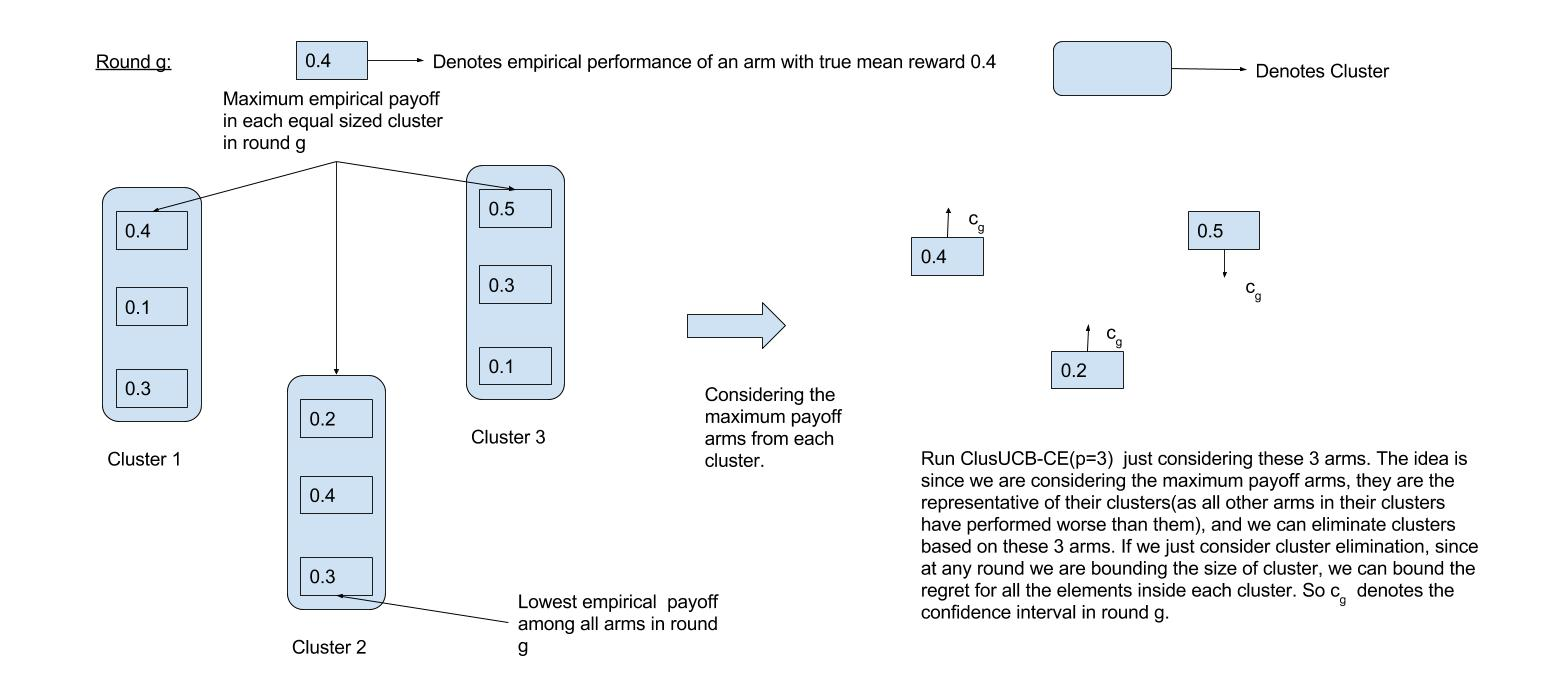
\includegraphics[scale=0.3]{img/diagCluster.jpg}
\caption{Cluster Elimination}
\end{figure}

\begin{proposition}
Considering only the cluster elimination condition, the total regret till $T$ is upper bounded by $R_{T}\leq \sum_{i\in A:\Delta_{i}\geq b}\bigg(\dfrac{2^{1+4\rho_{s}}\rho_{s}^{2\rho_{s}}T^{1-\rho_{s}}}{\Delta_{i}^{4\rho_{s}-1}}\bigg) + \bigg(\Delta_{i}+\dfrac{32(K+p)\rho_{s}\log{(T\dfrac{\Delta_{i}^{4}}{16\rho_{s}^{2}})}}{p\Delta_{i}}\bigg)  +  \bigg(\dfrac{T^{1-\rho_{s}}2^{2\rho_{s}+\frac{3}{2}}}{\Delta_{i}^{4\rho_{s} -1}} \bigg) \bigg \rbrace+\sum_{i\in A:0\leq\Delta_{i}\leq b}\bigg(\dfrac{T^{1-\rho_{s}}2^{2\rho_{s}+\frac{3}{2}}}{b^{4\rho_{s} -1}} \bigg) + max_{i:\Delta\leq b}\Delta_{i}T$, where $\rho_{s}\in (0,1)$, $p$ is the number of clusters and $T$ is the horizon.
\end{proposition}


\begin{remark} A sketch of the proof is given below,
\newline
\begin{itemize}
\item Define $g$-th round(in proposition 6) as the same way as the $m$-th round signifying the first/minimum round when a cluster gets eliminated.
\item Let in the $g$-th round $C_{g}$ be the set which contains all the max payoff arms from each cluster.
\item For regret bound proof according to proposition $5$, consider only this $C_{g}$ and proof following the same way as in proposition $5$ with some minor change. Hence, $C_{g}$ actually behaves like the set $B_{m}$ in proposition $5$ but contains just the max payoff arm from each cluster.
\item Introduce a bounded parameter $\rho_{s}\in (0,1]$ for cluster elimination to mimic the arm elimination condition in proposition $5$, but with the condition that whenever $\sqrt{\rho_{s}\epsilon_{g}}\leq \dfrac{\Delta_{i}}{2}, a_{i}\in C_{g}$, then the cluster $s_{k}$(where $\hat{r}_{i}$ is the max payoff) gets eliminated. Because of the algorithm, we are guaranteed that the size of the cluster in the $g$-th round is $\ell=\bigg\lceil \dfrac{K}{p}\bigg\rceil$.
\end{itemize}
\end{remark}

%\begin{remark} We also point out a few other observations:
%\newline
%\begin{itemize}
%\item The maximum number of clusters that can be formed in any round is $\big\lceil \dfrac{K}{2}\big\rceil$, since we start with a minimum cluster size of $\ell_{g}=2$.
%\item Also as $\epsilon_{g}$ decreases after every round and as $\epsilon_{g}\to \Delta, |S_{g}|\to D $, where $D$ is the true number of clusters based on the underlying distribution of $r_{i}, \forall i\in A$.
%\item On the implementation side, the subroutine SubroutineCluster(p) is implemented in such a way, that after arranging the arms in ascending order based on their $\hat{r}_{i}$, a sweep from left to right will put the arms in their respective clusters in such a way that $|\hat{r}_{i}-\hat{r}_{j}|,\forall i,j \in B_{g}$ is at most $\epsilon_{g}$. 
%\end{itemize}
%\end{remark}

\begin{proof} of Proposition 6:

Let $C_{g}=\lbrace \hat{r}_{max_{s_{i}}}| \forall s_{i}\in S \rbrace$, that is let $C_{g}$ be the set of all arms which has the maximum estimated payoff in their respective clusters in the $g$-th round.

Let, for each sub-optimal arm $a_{i}\in C_{g}$, $g_{i}=\min{\lbrace g|\sqrt{\rho_{s}\epsilon_{g}}\leq \dfrac{\Delta_{i}}{2} \rbrace}$. So, $g_{i}$ be the first round when $\sqrt{\rho_{s}\epsilon_{g}}\leq \dfrac{\Delta_{i}}{2}$ where $a_{i}\in C_{g}$ is the maximum payoff arm in cluster $s_{k}$. We will also consider that $\max \hat{r}_{i}\in C_{g}$ is $a^{*}$ and it has not still been eliminated. The parameter $\rho_{s}$ is introduced just to make sure that the cluster elimination is a more aggressive elimination than arm elimination.

So, for cluster elimination we will only be considering the arms in $C_{g}$ and following the proof of proposition $5$,

\subsection{Case a:} 
Some sub-optimal arm $a_{i}$ is not eliminated in round $g_{i}$ or before and the optimal arm $a^{*}\in B_{g_{i}} \subset B_{m_{i}}$
\newline In arm elimination condition, given the choice of confidence interval $c_{g}$, we want to bound the event $\hat{r}_{i}+c_{g_{i}}\leq \hat{r}^{*}-c_{g_{i}}$.
%with a more tighter event of $ \hat{r}_{i} + \sqrt{w_{s_{i}}}c_{m} \leq \hat{r}^{*} - \sqrt{w_{s_{i}}}c_{m}$ which will result in faster elimination of arms within a cluster, given the choice of $c_{m}$ and $w_{s_{i}}$.
\newline Now, $c_{g_{i}}=\sqrt{\dfrac{\rho_{s} \log (T\epsilon_{g_{i}}^{2})}{2 n_{g_{i}}}}$, where $0 < \rho_{s}\leq 1$
\newline Putting the value of $n_{g_{i}}=\dfrac{2\log{(T\epsilon_{g_{i}}^{2})}}{\epsilon_{g_{i}}}$ in $c_{g_{i}}$,
\newline $c_{g_{i}}=\sqrt{\dfrac{\rho_{s}*\epsilon_{g_{i}}\log (T\epsilon_{g_{i}}^{2})}{2*2 \log(T\epsilon_{g_{i}}^{2})}}=\sqrt{\dfrac{\rho_{s}\epsilon_{g_{i}}}{2}} = \sqrt{\rho_{s}\epsilon_{g_{i}+1}} < \dfrac{\sqrt{\rho_{s}}\Delta_{i}}{4} < \dfrac{\Delta_{i}}{4} $
%\leq\dfrac{\epsilon_{m}\sqrt{\ell_{m}}}{2\sqrt{w\ell_{m}}}\leq \dfrac{\epsilon_{m}}{2\sqrt{w}}$.
%\newline But in $\xi_{1}$, $\ell_{m}=2^{m}$.
%\newline Hence, $c\leq \dfrac{\epsilon_{m} 2^{m/2}}{4}$.
\newline Again, $\exists a_{i} \in C_{g}$ such that, 
$\hat{r}_{i} + c_{g_{i}}\leq r_{i} + 2c_{g_{i}} $
%\newline\hspace*{14em}$= \hat{r}_{i}-\sqrt{\epsilon_{m}} + 2c_{m} +\sqrt{\epsilon_{m}}$
\newline\hspace*{14em}$= \hat{r}_{i} + 4c_{g_{i}} - 2c_{g_{i}} $
\newline\hspace*{14em}$\leq r_{i} + \Delta_{i} - 2c_{g_{i}}$
\newline\hspace*{14em}$< r^{*} -2c_{g_{i}} $
\newline\hspace*{14em}$\leq \hat{r}^{*} - c_{g_{i}}$
%\newline\hspace*{14em}$= r_{i} + 5\dfrac{\sqrt{\epsilon_{m}}}{\sqrt{w_{s_{i}}}} - 2\sqrt{w_{s_{i}}}c_{m}$
%\newline \hspace*{4em}
%\newline But, $\epsilon_{m}=\dfrac{\hat{\Delta}_{s,m}}{\ell_{m}}$, where $\hat{\Delta}_{s,m}=\max_{i\in B_{m}}{\hat{r}_{i}}-\min_{j\in B_{m}}{\hat{r}_{j}},i\neq j$ and $\ell_{m}$ is increased after every round.
%\newline \hspace*{4em}$\leq \hat{r}_{i} + \epsilon_{m} 2^{(m-4)/2} - 2c$
\newline Hence, we get that as soon as $\sqrt{\rho_{s}\epsilon_{g_{i}}}<\dfrac{\Delta_{i}}{2}$, $\exists a_{i}\in C_{g}$ which gets eliminated.
%\newline So, $\hat{r}_{i}+c_{m}\leq \hat{r}_{i}+2c_{m}\leq r_{i} + \Delta_{i} - 2\sqrt{w_{s_{i}}}c_{m}\leq r^{*} - 2\sqrt{w_{s_{i}}}c_{m}$
%\leq \hat{r}^{*} - \sqrt{w}c_{m}
%\newline $\Rightarrow\hat{r}_{i}+c_{m}\leq \hat{r}_{i} - \sqrt{w}c_{m}  \leq r^{*} - \sqrt{w}c_{m}$
%\newline $\Rightarrow \hat{r}_{i} \leq {r}^{*} - 2\sqrt{w_{s_{i}}}c_{m} - 2c_{m} \leq \hat{r}^{*} - 2\sqrt{w_{s_{i}}}c_{m}$
\newline So, we need to bound the event of $\hat{r}_{i}+c_{g_{i}}\leq \hat{r}^{*}-c_{g_{i}}$ given that $\sqrt{\rho_{s}\epsilon_{g_{i}}}<\dfrac{\Delta_{i}}{2}$ becomes true for some arm $a_{i}\in C_{g}$ after the $g$-th round and $c_{g_{i}}=\sqrt{\dfrac{\rho_{s} \log (T\epsilon_{g_{i}}^{2})}{2 n_{g_{i}}}}$.
%\newline $\Rightarrow \hat{r}_{i}+2c_{m}\leq \hat{r}_{i} + 2\sqrt{w}c_{m} \leq \hat{r}^{*}$
%\newline $\Rightarrow \hat{r}_{i} + \sqrt{w}c_{m} \leq \hat{r}^{*} - \sqrt{w}c_{m}$
%\newline $\Rightarrow\hat{r}_{i}+c_{m}\sqrt{\dfrac{w\ell_{m}}{\epsilon_{m}}} \leq \hat{r}^{*}-c_{m}\sqrt{\dfrac{w\ell_{m}}{\epsilon_{m}}} $, as $c_{m}\sqrt{\dfrac{w\ell_{m}}{\epsilon_{m}}} > 0$

%\begin{proof} of Proposition 2:
%\newline
%Now, we can bound $\hat{r}_{i}+c_{m}\leq \hat{r}^{*}-c_{m}$ given that $\sqrt{\epsilon_{m}}<\dfrac{\Delta_{i}}{2}$ for some arm $a_{i}\in s_{i}$. 
	So, we need to bound the probability,
\newline\hspace*{4em} $\mathbb{P}\lbrace\hat{r}^{*}\leq r^{*} - c_{g_{i}}\rbrace\leq U_{g}$, where $U_{g}$ is an  arbitrary upper bound.
%, for a fixed $n_{s_{i}}$.
%\mathbb{P}\lbrace\hat{r}^{*}\leq r^{*} - c_{m}\rbrace\leq
\newline
%Here, we guarantee that only if $\hat{r}^{*}\leq r^{*} - c_{m}\sqrt{\dfrac{w\ell_{m}}{\epsilon_{m}}}$ or $\hat{r}_{i}\geq r_{i} + c_{m}\sqrt{\dfrac{w\ell_{m}}{\epsilon_{m}}}$ then only arm will not be deleted. This is a more aggressive arm elimination condition than simply looking at $\hat{r}^{*}\leq r^{*} - c_{m}$ or $\hat{r}_{i}\geq r_{i} + c_{m}$ because we are exploring much carefully by dividing the larger problem into sub-problems.
%\newline
Applying Chernoff-Hoeffding bound and considering independence of events,
\newline
\newline\hspace*{0em} $\mathbb{P}\lbrace\hat{r}^{*}\leq r^{*} - c_{g_{i}}\rbrace\leq exp(-2c_{g_{i}}^{2}n_{g_{i}})$
\newline\hspace*{8em} $\leq exp(-2 * \dfrac{\rho_{s}\log ( T\epsilon_{g_{i}}^{2})}{2 n_{g_{i}}} *n_{g_{i}})$
\newline\hspace*{8em} $\leq \dfrac{1}{(T\epsilon_{g_{i}}^{2})^{\rho_{s}}}$
%$\leq \bigg(\dfrac{1}{4\psi(m)T\epsilon_{m}^{2}}\bigg)^{D}$, as $\ell_{m}-1\leq D$
%\newline\hspace*{2em}
\newline
Similarly, $\mathbb{P}\lbrace\hat{r}_{i}\geq r_{i} + c_{g_{i}}\rbrace\leq \dfrac{1}{(T\epsilon_{g_{i}}^{2})^{\rho_{s}}}$
\newline
Summing, the two up, the probability that a sub-optimal arm $a_{i}\in C_{g}$ is not eliminated in $g_{i}$-th round is  $\bigg(\dfrac{2}{(T\epsilon_{g_{i}}^{2})^{\rho_{s}}}\bigg)$. 
\newline Now, for each round $g$, all the elements of $C_{g}$ are the respective max payoff arms of their cluster $s_{k}, \forall s_{k}\in S_{g}$, that is all the other arms in their respective clusters have performed worse than them. Hence, since $A\supset C_{g}$ and we can bound the max probability that a sub-optimal arm $a_{j}\in A$ is not eliminated in the $g$-th round by the same probability of $\bigg(\dfrac{2}{(T\epsilon_{g_{i}}^{2})^{\rho_{s}}}\bigg)$. 
\newline
Summing up over all arms in $A$ and bounding trivially by $T\Delta_{i}$,
\newline\hspace*{4em} $\sum_{i\in A}\bigg(\dfrac{2T\Delta_{i}}{(T\dfrac{\Delta_{i}}{16\rho_{s}^{2}}^{4})^{\rho_{s}}}\bigg)\leq \sum_{i\in A}\bigg(\dfrac{2^{1+4\rho_{s}}T^{1-\rho_{s}}\rho_{s}^{2\rho_{s}}\Delta_{i}}{\Delta_{i}^{4\rho_{s}}}\bigg)$
\newline\hspace*{12em}
$\leq \sum_{i\in A}\bigg(\dfrac{2^{1+4\rho_{s}}\rho_{s}^{2\rho_{s}}T^{1-\rho_{s}}}{\Delta_{i}^{4\rho_{s}-1}}\bigg)$
\newline Thus, we see that putting a value of $\rho_{s}=1$, nicely brings out the result of case b1 of proposition $5$.


\subsection{Case b1:} 
Either an arm $a_{i}\in C_{g}$ is eliminated along with all the arms in that cluster in round $g_{i}$(or before) or else there is no optimal arm $a^{*}\in C_{g_{i}}$. Again, in the $g$-th round, the maximum total elements in the cluster can be no more than $\ell=\bigg\lceil \dfrac{K}{p}\bigg\rceil$.
\newline
Also, since we are eliminating a sub-optimal arm $a_{i}\in C_{g_{i}}$ on or before round $g_{i}$, it is pulled (along with all the other arms in that cluster) no longer than,
\newline
\hspace*{4em}$n_{g_{i}}=\bigg\lceil\dfrac{2\log{(T\epsilon_{g_{i}}^{2})}}{\epsilon_{g_{i}}}\bigg\rceil$
\newline
%$\sqrt{\dfrac{\epsilon_{m}}{w}}<\dfrac{\Delta_{i}}{5}\Rightarrow \sqrt{\dfrac{\epsilon_{m}}{\ell_{m}^{2}}}<\dfrac{\Delta_{i}}{5}$, as $w\geq \ell_{m}^{2}$
%\newline
%$\Rightarrow \sqrt{\dfrac{\epsilon_{m}}{\ell_{m}^{2}}}<\dfrac{\Delta_{i}}{5}$
%\newline
So, the total contribution of $a_{i}$  along with all the other arms in the cluster till round $g_{i}$ is given by,
\newline
\hspace*{4em}$\Delta_{i}\bigg\lceil\dfrac{2\ell\log{(T\epsilon_{g_{i}}^{2})}}{\epsilon_{g_{i}}}\bigg\rceil$
%\newline
%\hspace*{4em}
$\leq\Delta_{i}\bigg\lceil\dfrac{2\ell\log{(T(\dfrac{\Delta_{i}}{2\sqrt{\rho_{s}}})^{4})}}{(\dfrac{\Delta_{i}}{2\sqrt{\rho_{s}}})^{2}}\bigg\rceil$, since $\sqrt{\rho_{s}\epsilon_{g_{i}}}\leq\dfrac{\Delta_{i}}{2}$
\newline
\hspace*{12em}
$\leq\Delta_{i}\bigg(1+\dfrac{32*(\frac{K}{p}+1)*\rho_{s}*\log{(T(\dfrac{\Delta_{i}}{2\sqrt{\rho_{s}}})^{4})}}{\Delta_{i}^{2}}\bigg)$, since in the $g$-th round the maximum cluster size is bounded by $\ell=\bigg\lceil \dfrac{K}{p} \bigg\rceil$.
\newline
\hspace*{12em}$\leq\Delta_{i}\bigg(1+\dfrac{32*(K+p)*\rho_{s}*\log{(T(\dfrac{\Delta_{i}}{2\sqrt{\rho_{s}}})^{4})}}{p\Delta_{i}^{2}}\bigg)$
\newline
\hspace*{12em}
$\leq\Delta_{i}\bigg(1+\dfrac{32(K+p)\rho_{s}\log{(T\dfrac{\Delta_{i}^{4}}{16\rho_{s}^{2}})}}{p\Delta_{i}^{2}}\bigg)$
\newline
Summing over all arms in $A \supset C_{g}$,
\newline
\hspace*{4em}$\leq\sum_{i\in A}\Delta_{i}\bigg(1+\dfrac{32\rho_{s}(K+p)\log{(T\dfrac{\Delta_{i}^{4}}{16\rho_{s}^{2}}})}{p\Delta_{i}^{2}}\bigg)$
\newline
%\hspace*{4em}$\leq\sum_{i\in B_{m}}\bigg(\Delta_{i}+\dfrac{27\log{(\psi(m)T\dfrac{\Delta_{i}^{\frac{8}{5}}}{12})}}{\Delta_{i}^{\frac{3}{5}}}\bigg)$
%\newline
%\hspace*{4em}$\leq\sum_{i\in B_{m}}\bigg(\Delta_{i}+\dfrac{12.5\log{(\psi(m)T\Delta_{i}^{4})}}{\Delta_{i}}\bigg)$
	%Thus, we see that the growth of the $n_{s_{i}}$ is always linear and not quadratic as in UCB-Revisited(\cite{auer2010ucb}). Also once $2l_{m}=D$, then $n_{s_{i}}$ will remain constant for the next rounds till stopping condition is met. Thus we have a more controlled exploration than UCB-Revisited(\cite{auer2010ucb}) and Median Elimination(\cite{even2006action}). Hence, 
%\newline
%\hspace*{4em}$\leq\sum_{i\in B_{m}}\bigg(\Delta_{i}+\dfrac{54\log{(\psi(m)T\dfrac{\Delta_{i}^{\frac{8}{5}}}{12})}}{\Delta_{i}^{\frac{3}{5}}}\bigg)$
%\newline
%But, $\psi(m)\leq c/m$ for any $c>0$ and so the regret upper bound comes off as 
%But, $\psi(m) = 1$ the regret upper bound comes off as 
%\newline
%$R_{T}\leq \sum_{i\in A}\bigg (\max{\bigg\lbrace \bigg(\dfrac{32}{(\Delta_{i})^{3}}\bigg) ,\bigg(\dfrac{25\Delta_{i}}{(\Delta^{2})(0.16T\Delta^{2})^{2|B_{m}|^{2}\Delta/5}}\bigg)\bigg\rbrace} + \bigg(\Delta_{i}+\dfrac{32\log{(T\dfrac{\Delta_{i}^{4}}{16})}}{\Delta_{i}}\bigg)\bigg)$. 
%\todo{will prove case b2 once you verify that this approach is correct}

\subsection{Case b2:} 
In this case we will consider that the cluster containing the optimal arm $a^{*}$ was eliminated by a sub-optimal cluster. Firstly, if conditions of case b1 holds then the optimal arm $a^{*}\in C_{g}$ will not be eliminated in round $g=g_{*}$ or it will lead to the contradiction that $r_{i}>r^{*}$ where $a_{i},a^{*}\in C_{g}$. In any round $g_{*}$, if the optimal arm $a^{*}$ gets eliminated then for any round from $1$ to $g_{j}$ all arms $a_{j}\in C_{g}$ such that $\sqrt{\rho_{s}\epsilon_{g}}<\dfrac{\Delta_{j}}{2}$ were eliminated according to assumption in case b1. Let, the arms surviving till $g_{*}$ round be denoted by $C_{g}^{'}$. This leaves any arm $a_{b}$ such that $\sqrt{\rho_{s}\epsilon_{g}}\geq\dfrac{\Delta_{b}}{2}$ to still survive and eliminate arm $a^{*}$ in round $g_{*}$. Let, such arms that survive $a^{*}$ belong to $C_{g}^{''}$. Also maximal regret per step after eliminating $a^{*}$ is the maximal $\Delta_{j}$ among the remaining arms $a_{j}$ with $g_{j}\geq g_{*}$.  Let $g_{b}$ be the round when $\sqrt{\rho_{s}\epsilon_{g}}<\dfrac{\Delta_{b}}{2}$ that is $g_{b}=min\lbrace g|\sqrt{\rho_{s}\epsilon_{g}}<\dfrac{\Delta_{b}}{2}\rbrace$. Hence, the maximal regret after eliminating the arm $a^{*}$ is upper bounded by, 
\newline
$\sum_{g_{*}=0}^{max_{j\in C_{g}^{'}}g_{j}}\sum_{i\in C_{g}^{''}:g_{i}>g_{*}}\bigg(\dfrac{2}{(T\epsilon_{g}^{2})^{\rho_{s}}} \bigg).T\max_{j\in C_{g}^{''}:g_{j}\geq g_{*}}{\Delta}_{j}$
\newline
But, we know that for any round $g$, elements of $C_{g}$ are the best performers in their respective clusters. So, taking that into account and $A'\supset C_{g}^{'}$ and $A''\supset C_{g}^{''}$
\newline
$\leq\sum_{g_{*}=0}^{max_{j\in A^{'}}g_{j}}\sum_{i\in A^{''}:g_{i}>g_{*}}\bigg(\dfrac{2}{(T\epsilon_{g}^{2})^{\rho_{s}}} \bigg).T\max_{j\in A^{''}:g_{j}\geq g_{*}}{\Delta}_{j}$
\newline
%$=\sum_{g_{*}=0}^{max_{j\in A^{'}}g_{j}}\sum_{i\in A^{''}:g_{i}>g_{*}}\bigg(\dfrac{2}{T\epsilon_{g}^{2}} \bigg).T\max_{j\in A^{''}:g_{j}\geq g_{*}}{\Delta}_{j}$
%\newline
\hspace*{0em}$\leq\sum_{g_{*}=0}^{max_{j\in A^{'}}g_{j}}\sum_{i\in A^{''}:g_{i}>g_{*}}\bigg(\dfrac{2}{(T\epsilon_{g}^{2})^{\rho_{s}}} \bigg).T.2\sqrt{\rho_{s}\epsilon_{g}}$, since $\sqrt{\rho_{s}\epsilon_{g}}<\dfrac{\Delta_{i}}{2}$
\newline
\hspace*{0em}$\leq\sum_{g_{*}=0}^{max_{j\in A^{'}}g_{j}}\sum_{i\in A^{''}:g_{i}>g_{*}}\bigg(\dfrac{4 T^{1-\rho_{s}}}{\epsilon_{g}^{2\rho_{s} - \frac{1}{2}}} \bigg) $
%\newline
%\hspace*{0em}$\leq\sum_{m_{*}=0}^{max_{j\in A^{'}}m_{j}}\sum_{i\in A^{''}:m_{i}>m_{*}}\bigg(\dfrac{4.4^{3/2}}{\Delta_{i}^{3}} \bigg) $, as $\sqrt{\epsilon_{m}}\leq\dfrac{\Delta_{i}}{2}$
\newline
\hspace*{0em}$\leq\sum_{i\in A^{''}:g_{i}>g_{*}}\sum_{g_{*}=0}^{\min{\lbrace g_{i},g_{b}\rbrace}}\bigg(\dfrac{4T^{1-\rho_{s}}}{2^{({2\rho_{s} - \frac{1}{2}})g_{*}}} \bigg) $
\newline
\hspace*{0em}$\leq\sum_{i\in A^{'}}\bigg(\dfrac{4T^{1-\rho_{s}}}{2^{({2\rho_{s} - \frac{1}{2}})g_{*}}} \bigg)+\sum_{i\in A^{''}\setminus A^{'}}\bigg(\dfrac{4T^{1-\rho_{s}}}{2^{({2\rho_{s} - \frac{1}{2}})g_{b}}} \bigg)$
%\newline
%\hspace*{0em}$<\sum_{i\in A^{'}}\bigg(4*2^{-(3/2)m_{*}} \bigg)+\sum_{i\in A^{''}\setminus A^{'}}\bigg(4*2^{-(3/2)m_{b}} \bigg)$
\newline
\hspace*{0em}$\leq\sum_{i\in A^{'}}\bigg(\dfrac{4T^{1-\rho_{s}}*2^{2\rho_{s}-\frac{1}{2}}}{\Delta_{i}^{4\rho_{s}-1}} \bigg)+\sum_{i\in A^{''}\setminus A^{'}}\bigg(\dfrac{4T^{1-\rho_{s}}*2^{2\rho_{s}-\frac{1}{2}}}{b^{4\rho_{s}-1}} \bigg)$
\newline
\hspace*{0em}$\leq\sum_{i\in A^{'}}\bigg(\dfrac{T^{1-\rho_{s}}2^{2\rho_{s}+\frac{3}{2}}}{\Delta_{i}^{4\rho_{s}-1}} \bigg)+\sum_{i\in A^{''}\setminus A^{'}}\bigg(\dfrac{T^{1-\rho_{s}}2^{2\rho_{s}+\frac{3}{2}}}{b^{4\rho_{s}-1}} \bigg)$
\newline
Summing up \textbf{Case a} and \textbf{Case b1} and \textbf{Case b2}, the total regret till round $g$ is given by,
\newline $R_{T}\leq \sum_{i\in A:\Delta_{i}\geq b}\bigg(\dfrac{2^{1+4\rho_{s}}\rho_{s}^{2\rho_{s}}T^{1-\rho_{s}}}{\Delta_{i}^{4\rho_{s}-1}}\bigg) + \bigg(\Delta_{i}+\dfrac{32(K+p)\rho_{s}\log{(T\dfrac{\Delta_{i}^{4}}{16\rho_{s}^{2}})}}{p\Delta_{i}}\bigg)  +  \bigg(\dfrac{T^{1-\rho_{s}}2^{2\rho_{s}+\frac{3}{2}}}{\Delta_{i}^{4\rho_{s} -1}} \bigg) \bigg \rbrace+\sum_{i\in A:0\leq\Delta_{i}\leq b}\bigg(\dfrac{T^{1-\rho_{s}}2^{2\rho_{s}+\frac{3}{2}}}{b^{4\rho_{s} -1}} \bigg) + max_{i:\Delta\leq b}\Delta_{i}T$


\end{proof}
\par Again, we see that $\rho_{s}=1$ and $p=K$(that is each arm is in a cluster of its own and so $\bigg\lceil \dfrac{K}{p} \bigg\rceil=1$) brings out a near equivalent result as the result of proposition $5$. That is, for $\rho_{s}=1,p=K$,
\newline $R_{T}\leq \sum_{i\in A:\Delta_{i}\geq b}\bigg \lbrace \bigg(\dfrac{44}{(\Delta_{i})^{3}}\bigg) + \bigg(\Delta_{i}+\dfrac{32\log{(T\dfrac{\Delta_{i}^{4}}{16})}}{\Delta_{i}}\bigg)\bigg\rbrace + \sum_{i\in A:0\leq\Delta_{i}\leq b}\dfrac{12}{b^{3}} + max_{i:\Delta\leq b}\Delta_{i}T$
\newline So, the most significant term for cluster elimination that is $\dfrac{32(K+p)\log{(T\dfrac{\Delta_{i}^{4}}{16})}}{p\Delta_{i}}$ is slightly more than arm elimination most significant term $\dfrac{32\log{(T\dfrac{\Delta_{i}^{4}}{16})}}{\Delta_{i}}$ because of the factor $\dfrac{K+p}{p}$, but its order is nearly same as arm elimination regret bound.
\par The principal takeaway from this result is that a lower value of $\rho_{s}\in (0,1]$ makes the algorithm risky(by increasing the error bound), but reduces expected regret whereas a higher value of $\rho_{s} > 1$ actually makes the algorithm less risky but at a cost of higher expected regret. The risk stems from the fact that the probability of sub-optimal arm elimination increases without proper exploration. So, there is always this trade-off between exploration and risk. So, in our algorithm we decrease the $\rho_{s}$ in a graded fashion halving after every round but $\rho_{s}$ is always bounded that is, $\rho \in (0,1)$. \

\begin{remark}
Considering, $\rho_{a}\in (0,1]$ interval, the regret upper bound for arm elimination can be modified in the same way giving us a bound of
\newline
$R_{T}\leq \sum_{i\in A:\Delta_{i}\geq b}\bigg(\dfrac{2^{1+4\rho_{a}}\rho_{a}^{2\rho_{a}}T^{1-\rho_{a}}}{\Delta_{i}^{4\rho_{a}-1}}\bigg) + \bigg(\Delta_{i}+\dfrac{32\rho_{a}\log{(T\dfrac{\Delta_{i}^{4}}{16\rho_{a}^{2}})}}{\Delta_{i}}\bigg)  +  \bigg(\dfrac{T^{1-\rho_{a}}2^{2\rho_{a}+\frac{3}{2}}}{\Delta_{i}^{4\rho_{a} -1}} \bigg) \bigg \rbrace+$\newline$\sum_{i\in A:0\leq\Delta_{i}\leq b}\bigg(\dfrac{T^{1-\rho_{a}}2^{2\rho_{a}+\frac{3}{2}}}{b^{4\rho_{a} -1}} \bigg) + max_{i:\Delta\leq b}\Delta_{i}T$. 
\newline
Putting $\rho_{a}=1$ gives us directly the result of proposition $3$.
\end{remark}

\section{Appendix C}

\begin{theorem}
Considering both the arm elimination and cluster elimination condition, the total regret till $T$ is upper bounded by $R_{T}\leq \sum_{i\in A:\Delta\geq b} \bigg\lbrace 2\Delta_{i}+ \bigg(\dfrac{44}{\Delta_{i}^{3}}\bigg) + \bigg(\dfrac{2^{1+4\rho_{s}}\rho_{s}^{2\rho_{s}}T^{1-\rho_{s}}}{\Delta_{i}^{4\rho_{s}-1}}\bigg) + \bigg(\dfrac{32\log{(T\dfrac{\Delta_{i}^{4}}{16})}}{\Delta_{i}}\bigg) + \bigg(\dfrac{32(K+p)\rho_{s}\log{(T\dfrac{\Delta_{i}^{4}}{16\rho_{s}^{2}})}}{p\Delta_{i}}\bigg)\bigg\rbrace + \sum_{i\in A:0\leq\Delta_{i}\leq b}\bigg\lbrace \bigg(\dfrac{12}{b^{3}} \bigg) + \bigg(\dfrac{T^{1-\rho_{s}}2^{2\rho_{s}+\frac{3}{2}}}{\Delta_{i}^{3}} \bigg)+\bigg(\dfrac{T^{1-\rho_{s}}2^{2\rho_{s}+\frac{3}{2}}}{b^{4\rho_{s} -1}} \bigg) \bigg\rbrace + max_{i:\Delta\leq b}\Delta_{i}T $, where $\rho_{s}\in (0,1]$, $p$ is the number of clusters and $T$ is the horizon.
\end{theorem}

\begin{proof}
Combining both the cases of Proposition $5$ and Proposition $6$ we can see that a sub-optimal arm $a_{i}$ can only be eliminated given that either $m_{i}$ or $g_{i}$ happens. In Proposition $5$ we consider only arm elimination and in Proposition $6$ we consider only cluster elimination. One vital point we point out is that, $\epsilon_{m}$(in proposition $5$) = $\epsilon_{g}$(in proposition $6$. Also we cluster the arms based on $\epsilon_{m}$.
\subsection{Case a:} 
So, we take the summation of the two events mentioned in Proposition $5$(case a) and Proposition $6$(case a)
which gives us an upper bound on the regret given that the optimal arm $a^{*}$ is still surviving, 
\newline
$\leq \sum_{i\in A}\bigg\lbrace\bigg(\dfrac{32}{\Delta_{i}^{3}}\bigg) + \bigg(\dfrac{2^{1+4\rho_{s}}\rho_{s}^{2\rho_{s}}T^{1-\rho_{s}}}{\Delta_{i}^{4\rho_{s}-1}}\bigg)\bigg\rbrace$ 
\newline
before a sub-optimal arm is eliminated by arm elimination or cluster elimination condition.
\subsection{Case b1:} 
Again, combining Proposition $5$(case b1) and Proposition $6$(case b1), we can show that till an arm or a cluster is eliminated, the maximum regret suffered due to pulling of a sub-optimal arm(or a sub-optimal cluster) is no less than,
\newline
$\sum_{i\in A}\bigg\lbrace\bigg(\Delta_{i}+\dfrac{32\log{(T\dfrac{\Delta_{i}^{4}}{16})}}{\Delta_{i}}\bigg) + \bigg(\Delta_{i}+\dfrac{32(K+p)\rho_{s}\log{(T\dfrac{\Delta_{i}^{4}}{16\rho_{s}^{2}})}}{p\Delta_{i}}\bigg)\bigg\rbrace $
\newline
\subsection{Case b2:} 
Lastly we have to take into consideration the error bound, that the optimal arm $a^{*}$ or the optimal cluster(that is the cluster containing the arm $a^{*}$) gets eliminated. Combining Proposition $5$(case b2) and Proposition $6$(case b2), we can show,
\newline
$\leq\sum_{i\in A^{'}}\bigg(\dfrac{12}{\Delta_{i}^{3}} \bigg)+\sum_{i\in A^{''}\setminus A^{'}}\bigg(\dfrac{12}{b^{3}} \bigg) + \sum_{i\in A^{'}}\bigg(\dfrac{T^{1-\rho_{s}}2^{2\rho_{s}+\frac{3}{2}}}{\Delta_{i}^{3}} \bigg)+\sum_{i\in A^{''}\setminus A^{'}}\bigg(\dfrac{T^{1-\rho_{s}}2^{2\rho_{s}+\frac{3}{2}}}{b^{4\rho_{s} -1}} \bigg)$
\newline
%Summing over all arms in $A$,
%\newline
%$\leq \sum_{i\in A} \bigg\lbrace\bigg(\Delta_{i}+\dfrac{32\log{(T\dfrac{\Delta_{i}^{4}}{16})}}{\Delta_{i}}\bigg) + \bigg(\Delta_{i}+\dfrac{512\rho_{s}\log{(T\dfrac{\Delta_{i}^{4}}{16\rho_{s}^{2}})}}{\Delta_{i}}\bigg)\bigg\rbrace $
%\newline
Hence, the total regret by combining \textbf{case a}, \textbf{case b1} and \textbf{case b2} is given by,
\newline
$R_{T}\leq \sum_{i\in A:\Delta\geq b} \bigg\lbrace \bigg(\dfrac{32}{\Delta_{i}^{3}}\bigg) + \bigg(\dfrac{2^{1+4\rho_{s}}\rho_{s}^{2\rho_{s}}T^{1-\rho_{s}}}{\Delta_{i}^{4\rho_{s}-1}}\bigg) + \bigg(\Delta_{i}+\dfrac{32\log{(T\dfrac{\Delta_{i}^{4}}{16})}}{\Delta_{i}}\bigg) + \bigg(\Delta_{i}+\dfrac{32(K+p)\rho_{s}\log{(T\dfrac{\Delta_{i}^{4}}{16\rho_{s}^{2}})}}{p\Delta_{i}}\bigg)\bigg\rbrace + \sum_{i\in A:0\leq\Delta_{i}\leq b}\bigg\lbrace \bigg(\dfrac{12}{\Delta_{i}^{3}} \bigg) + \bigg(\dfrac{12}{b^{3}} \bigg) + \bigg(\dfrac{T^{1-\rho_{s}}2^{2\rho_{s}+\frac{3}{2}}}{\Delta_{i}^{3}} \bigg)+\bigg(\dfrac{T^{1-\rho_{s}}2^{2\rho_{s}+\frac{3}{2}}}{b^{4\rho_{s} -1}} \bigg) \bigg\rbrace + max_{i:\Delta\leq b}\Delta_{i}T $
\newline
$R_{T}= \sum_{i\in A:\Delta\geq b} \bigg\lbrace 2\Delta_{i}+ \bigg(\dfrac{44}{\Delta_{i}^{3}}\bigg) + \bigg(\dfrac{2^{1+4\rho_{s}}\rho_{s}^{2\rho_{s}}T^{1-\rho_{s}}}{\Delta_{i}^{4\rho_{s}-1}}\bigg) + \bigg(\dfrac{32\log{(T\dfrac{\Delta_{i}^{4}}{16})}}{\Delta_{i}}\bigg) + \bigg(\dfrac{32(K+p)\rho_{s}\log{(T\dfrac{\Delta_{i}^{4}}{16\rho_{s}^{2}})}}{p\Delta_{i}}\bigg)\bigg\rbrace + \sum_{i\in A:0\leq\Delta_{i}\leq b}\bigg\lbrace \bigg(\dfrac{12}{b^{3}} \bigg) + \bigg(\dfrac{T^{1-\rho_{s}}2^{2\rho_{s}+\frac{3}{2}}}{\Delta_{i}^{3}} \bigg)+\bigg(\dfrac{T^{1-\rho_{s}}2^{2\rho_{s}+\frac{3}{2}}}{b^{4\rho_{s} -1}} \bigg) \bigg\rbrace + max_{i:\Delta\leq b}\Delta_{i}T $
%\newline
%Considering the case that all the arms are pulled once at the start,
%\newline
%$R_{T}\leq \sum_{i\in A:\Delta\geq b} \bigg\lbrace 3\Delta_{i}+ \bigg(\dfrac{44}{\Delta_{i}^{3}}\bigg) + \bigg(\dfrac{2^{1+4\rho_{s}}\rho_{s}^{2\rho_{s}}T^{1-\rho_{s}}}{\Delta_{i}^{4\rho_{s}-1}}\bigg) + \bigg(\dfrac{32\log{(T\dfrac{\Delta_{i}^{4}}{16})}}{\Delta_{i}}\bigg) + \bigg(\dfrac{32(K+p)\rho_{s}\log{(T\dfrac{\Delta_{i}^{4}}{16\rho_{s}^{2}})}}{p\Delta_{i}}\bigg)\bigg\rbrace + \sum_{i\in A:0\leq\Delta_{i}\leq b}\bigg\lbrace \bigg(\dfrac{12}{b^{3}} \bigg) + \bigg(\dfrac{T^{1-\rho_{s}}2^{2\rho_{s}+\frac{3}{2}}}{\Delta_{i}^{3}} \bigg)+\bigg(\dfrac{T^{1-\rho_{s}}2^{2\rho_{s}+\frac{3}{2}}}{b^{4\rho_{s} -1}} \bigg) \bigg\rbrace + max_{i:\Delta\leq b}\Delta_{i}T $
%\newline
%$R_{T}\leq \sum_{i\in A} \bigg\lbrace 2\Delta_{i}+\bigg(\dfrac{32}{\Delta_{i}^{3}}\bigg) + \bigg((2)^{8-4\rho_{s}}(\Delta_{i})^{1-4\rho_{s}}\rho_{s}^{2\rho_{s}}(T)^{1-\rho_{s}}\bigg) + \bigg(\dfrac{32\log{(T\dfrac{\Delta_{i}^{4}}{16})}}{\Delta_{i}}\bigg) + \bigg(\dfrac{512\rho_{s}\log{(T\dfrac{\Delta_{i}^{4}}{16\rho_{s}^{2}})}}{\Delta_{i}}\bigg)\bigg\rbrace $
\end{proof}

\begin{remark}
Considering the case when $\rho_{a}\in (0,1]$, the total regret bound can be rewritten as $R_{T}\leq \sum_{i\in A:\Delta\geq b} \bigg\lbrace \bigg(\bigg(\dfrac{2^{1+4\rho_{a}}\rho_{a}^{2\rho_{a}}T^{1-\rho_{a}}}{\Delta_{i}^{4\rho_{a}-1}}\bigg) + \bigg(\dfrac{2^{1+4\rho_{s}}\rho_{s}^{2\rho_{s}}T^{1-\rho_{s}}}{\Delta_{i}^{4\rho_{s}-1}}\bigg) + \bigg(\Delta_{i}+\dfrac{32\rho_{a}\log{(T\dfrac{\Delta_{i}^{4}}{16\rho_{a}^{2}})}}{\Delta_{i}}\bigg) +$ \newline $ + \bigg(\Delta_{i}+\dfrac{32(K+p)\rho_{s}\log{(T\dfrac{\Delta_{i}^{4}}{16\rho_{s}^{2}})}}{p\Delta_{i}}\bigg)\bigg\rbrace + \sum_{i\in A:0\leq\Delta_{i}\leq b}\bigg\lbrace \bigg(\dfrac{12}{b^{3}} \bigg) + \bigg(\dfrac{T^{1-\rho_{a}}2^{2\rho_{a}+\frac{3}{2}}}{\Delta_{i}^{3}} \bigg)+\bigg(\dfrac{T^{1-\rho_{a}}2^{2\rho_{a}+\frac{3}{2}}}{b^{4\rho_{a} -1}} \bigg) + \bigg(\dfrac{12}{b^{3}} \bigg) + \bigg(\dfrac{T^{1-\rho_{s}}2^{2\rho_{s}+\frac{3}{2}}}{\Delta_{i}^{3}} \bigg)+\bigg(\dfrac{T^{1-\rho_{s}}2^{2\rho_{s}+\frac{3}{2}}}{b^{4\rho_{s} -1}} \bigg) \bigg\rbrace + max_{i:\Delta\leq b}\Delta_{i}T   =    \sum_{i\in A:\Delta\geq b} \bigg\lbrace \bigg(\bigg(\dfrac{2^{1+4\rho_{a}}\rho_{a}^{2\rho_{a}}T^{1-\rho_{a}}}{\Delta_{i}^{4\rho_{a}-1}}\bigg) + \bigg(\dfrac{2^{1+4\rho_{s}}\rho_{s}^{2\rho_{s}}T^{1-\rho_{s}}}{\Delta_{i}^{4\rho_{s}-1}}\bigg) + \bigg(\Delta_{i}+\dfrac{32\rho_{a}\log{(T\dfrac{\Delta_{i}^{4}}{16\rho_{a}^{2}})}}{\Delta_{i}}\bigg) +$ \newline $ + \bigg(\Delta_{i}+\dfrac{32(K+p)\rho_{s}\log{(T\dfrac{\Delta_{i}^{4}}{16\rho_{s}^{2}})}}{p\Delta_{i}}\bigg)\bigg\rbrace + \sum_{i\in A:0\leq\Delta_{i}\leq b}\bigg\lbrace \bigg(\dfrac{24}{b^{3}} \bigg) + \bigg(\dfrac{T^{1-\rho_{a}}2^{2\rho_{a}+\frac{3}{2}}}{\Delta_{i}^{3}} \bigg)+\bigg(\dfrac{T^{1-\rho_{a}}2^{2\rho_{a}+\frac{3}{2}}}{b^{4\rho_{a} -1}} \bigg) + \bigg(\dfrac{T^{1-\rho_{s}}2^{2\rho_{s}+\frac{3}{2}}}{\Delta_{i}^{3}} \bigg)+\bigg(\dfrac{T^{1-\rho_{s}}2^{2\rho_{s}+\frac{3}{2}}}{b^{4\rho_{s} -1}} \bigg) \bigg\rbrace + max_{i:\Delta\leq b}\Delta_{i}T $ which follows directly from Proposition 1,2 and Theorem 1.

	So we see that the most significant term in the regret is the $\bigg(K\dfrac{32(K+p)\rho_{s}\log{(T\dfrac{\Delta_{i}^{4}}{16\rho_{s}^{2}})}}{p\Delta_{i}}\bigg)$. Also, its evident from the result that different values of $\rho_{a}$ and $\rho_{s}$ affects the regret bound differently. When $K$ is large and $p$ is small it is advantageous to run $\rho_{a}< \rho_{s}$ for any round $m$. This will aggressively eliminate arms within cluster while cluster elimination will be more conservative since each cluster will contain a large number of arms it is a good idea to eliminate clusters in the later rounds when sufficient exploration has been done.
	
\end{remark}

\section{Appendix D}

In this section we discuss about the various exploration regulatory function that we can use to control exploration. A similar topic has already been handled in \cite{liu2016modification} where they have introduced mainly three types of regulatory factors to the term $\bigg\lbrace\hat{r}_{i}+\sqrt{\dfrac{d_{i}\log T\tilde{\Delta}_{m}^{2}}{2n_{m}}}\bigg\rbrace$ which is used for selecting an arbitrary arm $a_{i}$ in the $t$-th timestep which maximizes the above term. This regulatory term $d_{i}$ can be of the form as $\dfrac{T}{t_{i}}$, $\dfrac{\sqrt{T}}{t_{i}}$ and $\dfrac{\log T}{t_{i}}$, where $t_{i}$ is the number of times an arm $a_{i}$ is sampled. One has to choose a regulatory factor based on how fast the algorithm should taper its exploration in the later rounds since with time, $t_{i}$ increases and only the numerator decides how fast the exploration must decrease.

	We also deploy a similar exploration regulatory factor called $\psi(m)=\dfrac{\sqrt{\log T}}{m+1}$ or $\dfrac{\log T}{m+1}$, where $m$ is the round. Depending on how fast the exploration must reduce we might choose any one of them. So $\psi(m)$ is dependent on round as opposed to each timestep or the number of times an individual arm is sampled as done in \cite{liu2016modification}. Also as $m$ increases, $\psi(m)$ decreases and we have a tapered exploration. We also point out that now our number of pulls becomes $n_{m}=\bigg\lceil\dfrac{2\log{(\psi(m)T\epsilon_{m}^{2})}}{\epsilon_{m}}\bigg\rceil$ and both the arm elimination and cluster elimination confidence interval becomes $\sqrt{\dfrac{\rho_{a}\log{(\psi(m)T\epsilon_{m}^{2})}}{2 n_{m}}}$ and $\sqrt{\dfrac{\rho_{s} \log{(\psi(m)T\epsilon_{m}^{2})}}{2 n_{m}}}$  respectively. The rest of the theoretical analysis remains unchanged. 
	
	But this $\psi(m)=\dfrac{\log T}{m+1}$ significantly affects two factors, the regret suffered for arm and cluster elimination and the error bound. In the first case, it becomes $ \sum_{i\in A}\bigg\lbrace\bigg(\dfrac{32}{(log T)\Delta_{i}^{3}}\bigg) + \bigg(\dfrac{2^{1+4\rho}\rho^{2\rho}T^{1-\rho}}{(\log T)\Delta_{i}^{4\rho-1}}\bigg)\bigg\rbrace$ from case a) in Theorem 1 and $\sum_{i\in A^{'}}\bigg(\dfrac{12}{(\log T)\Delta_{i}^{3}} \bigg)+\sum_{i\in A^{''}\setminus A^{'}}\bigg(\dfrac{12}{(\log T) b^{3}} \bigg) + \sum_{i\in A^{'}}\bigg(\dfrac{T^{1-\rho}2^{2\rho+\frac{3}{2}}}{(\log T) \Delta_{i}^{3}} \bigg)+\sum_{i\in A^{''}\setminus A^{'}}\bigg(\dfrac{T^{1-\rho}2^{2\rho+\frac{3}{2}}}{(\log T) b^{4\rho -1}} \bigg)$ from case b2) in Theorem 1. So, in both the cases we see that the exploratory regulatory factor actually decreases our risk by decreasing the error bound and at the same time increases the probability of arm or cluster elimination. 
	
	For the main regret contributing term $\bigg(\dfrac{32(K+p)\rho\log{(\psi(m)T\dfrac{\Delta_{i}^{4}}{16\rho^{2}})}}{p\Delta_{i}}\bigg) \leq \bigg(\dfrac{32(K+p)\rho\log{(T\dfrac{\Delta_{i}^{4}}{16\rho^{2}}\log T)}}{p\Delta_{i}}\bigg)$ , the $\log \log T$ term is nearly negligible and only slightly increase the expected regret.


\section{Appendix E}
%\begin{table}
%\caption{Regret Upper Bound of Algorithms}
\label{sample-table}
\begin{center}
\begin{tabular}{ll}
\multicolumn{1}{c}{\bf Algorithm}  &\multicolumn{1}{c}{\bf Cumulative Regret Upper Bound} \\
\hline \\
UCB1         &\hspace*{5em}$\min\bigg\lbrace O(\sqrt{KT\log T}) ,O\bigg(\dfrac{K\log T}{\Delta}\bigg)\bigg\rbrace$ \\
UCB2         &\hspace*{5em}$O\bigg(K\bigg(\dfrac{(1 + \epsilon(\alpha)) log(T)}{2\Delta} + C(\alpha)\bigg)\bigg)$, $0<\alpha<1$ \\
$\epsilon_{n}$-greedy         &\hspace*{5em}$O\bigg(\dfrac{K\Delta\log T}{d^{2}}\bigg)$, $0<d<\Delta$ \\
EXP3             &\hspace*{5em}$O\bigg(S \sqrt{KT \log(KT)}\bigg)$, where $S$ is the hardness of the problem \\
UCB($\delta$)	&\hspace*{5em}$O\bigg(\dfrac{16K}{\Delta}\log\big(\dfrac{2K}{\Delta\delta}\big)\bigg)$ , where $\delta$ is the error probability\\
UCB-Revisited             &\hspace*{5em}$\min\bigg\lbrace O(\sqrt{KT}\dfrac{log(K\log K)}{\sqrt{K}}), O\bigg(\dfrac{K\log (T\Delta^{2})}{\Delta}\bigg)\bigg\rbrace$ \\
MOSS				&\hspace*{5em}$\min\bigg\lbrace O\bigg(\sqrt{KT}\bigg), O\bigg(\dfrac{K\log(T\Delta^{2}/K)}{\Delta}\bigg) \bigg \rbrace$\\
KL-UCB         &\hspace*{5em}$O\bigg(K\bigg(\dfrac{\Delta \log(T)(1 + \epsilon)}{d(r_{i}, r^{*} )} + \log(\log(T)) + \dfrac{(\epsilon)}{T^{\beta(\epsilon)}}\bigg)\bigg)$, where $\epsilon > 0$ and $d(r_{i}, r^{*})>2\Delta_{i}^{2}$\\
UCB-Clustered             &\hspace*{5em}$\min\bigg\lbrace\dfrac{\sqrt{KT}\log{(\dfrac{K^{4}(\log K)^{2}}{T})}}{\sqrt{\log K}},O\bigg(\dfrac{(K+p)K\log (T\Delta^{4})}{p\Delta}\bigg)\bigg\rbrace$, \\& \hspace*{5em} where $p$ is the number of clusters \\
%Clustered-UCB         &$O\bigg(K\bigg (\max{\bigg\lbrace \bigg(\dfrac{1}{\psi(m)(\Delta)^{\frac{3}{5}}}\bigg) ,\bigg(\dfrac{\Delta}{(\psi(m)\Delta^{2})(\psi(m)T\Delta^{2})^{2K^{2}\Delta/5}}\bigg)\bigg\rbrace}$\\&$ + \bigg(\Delta +\dfrac{\log{(\psi(m)T\Delta^{\frac{8}{5}})}}{\Delta^{\frac{3}{5}}}\bigg)\bigg)\bigg)$, let $\psi(m)=\dfrac{c}{m},c>0$ \\
\end{tabular}
\end{center}
%\end{table}


